\section{EnergyPlus based simulation for smart buildings}
\label{sec:energy_plus_review}
In this section, we review the EnergyPlus software program, which provides
accurate input and output traces from buildings for validation of the new
thermal modeling algorithms.

EnergyPlus software package is a suite of algorithms that calculate the
energy required to operate a building and its resulting thermal behavior based
on numerous considerations ranging from the specifications of the structure, to
heat sources and sinks within the building. EnergyPlus consists of
an integrated solution manager that manages the calculation of the heat balance
of various surfaces in a simulated building, its mechanical systems, and the air.
The solutions to each of these three elements
are calculated separately and loosely coupled to each other using the manager at
each time-step. Due to its modularity, it is easy to establish links to other
programs such as Google SketchUp for 3D modeling and visualization.
EnergyPlus has been proven as a successful energy
simulation program with widely-accepted accuracy for modern buildings
\cite{yang2016review}: among all its applications, for instance, it has been
used as a kernel of high level building energy and control systems test bed
\cite{wetter2011co}, and a key validation tool of an energy saving model
\cite{mardaljevic2009daylight}. Instead of conducting real building
experiments, using EnergyPlus to test and simulate the proposed models is
therefore valid, with a state of art simulation accuracy, which was a major
pain point in the past. On the other hand, using EnergyPlus allows the authors
to efficiently choose from a variety of buildings to test on, and to easily
configure energy inputs.

An input data file (IDF) and a weather file are needed for the EnergyPlus
simulation. The IDF includes all the information of the building such
as size, structure, position and the HVAC subsystem, etc. The IDF
editor in EnergyPlus can be used to change parameters of the building, the
schedule of the HVAC subsystem and also the output information. The
selected output information is generated in the spreadsheet file
after running the simulation.

Fig.~\ref{fig:5zone} shows the side view of an office building
with 5 rooms and HVAC modeled in EnergyPlus. The heat sources for this building
can be HVAC, light, occupants, electric equipment, air filtration, etc. The
room temperature is also affected by the weather (ambient temperature and solar
factors) and can be controlled by the HVAC system with coils
and fans.

\begin{figure}[t]
    \centering
    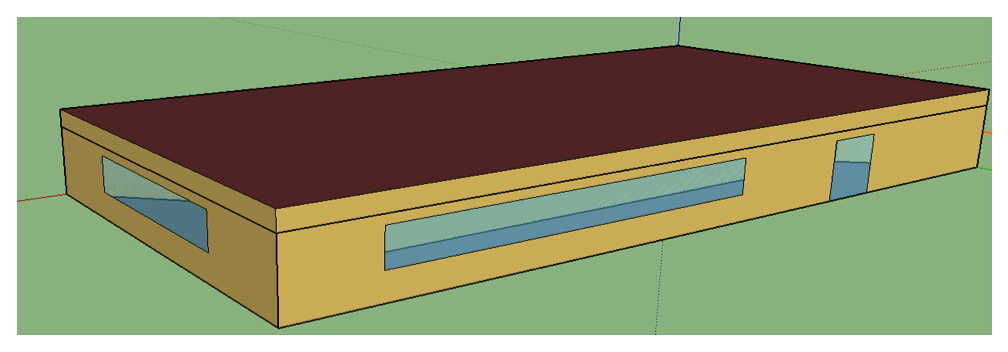
\includegraphics[width=0.7\columnwidth]{figs/energyplus_review/5zone-a}
    \caption{Side view of a 5-zone office building}
    \label{fig:5zone}
\end{figure}

Fig.~\ref{fig:energyplus-io-curve} shows the simulated temperature changes and
input changes over 15 days from EnergyPlus for an office building with the 5 zones
(rooms), as shown in Fig.~\ref{fig:5zone}. EnergyPlus can assign different schedules
for each room while simulating the thermal model.
Fig.~\ref{fig:occupancy-curve} shows a typical working schedule of the 5-room
office building.

\begin{figure}[t]
    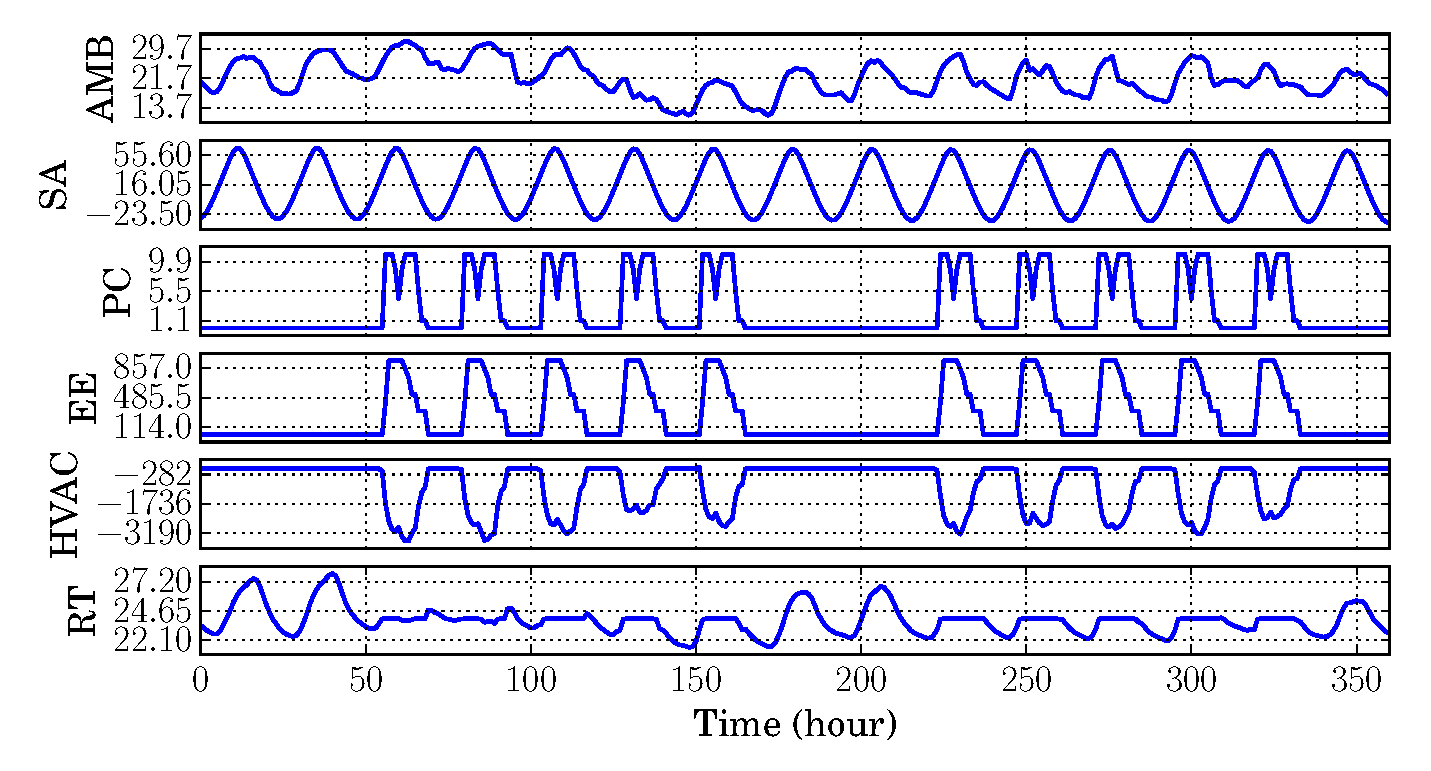
\includegraphics[width=0.9\columnwidth]{figs/energyplus_review/energyplus}
    \caption{Selected EnergyPlus input and simulated temperature output data sample in
        15 days.  (AMB: AMBient temperature; SA: Solar angle; PC: People count
        (occupancy); EE: Electrical equipment power; HVAC: HVAC system
        cooling/heating power; RT: Room Temperature)}
    \label{fig:energyplus-io-curve}
\end{figure}
\begin{figure}[t]
\centering
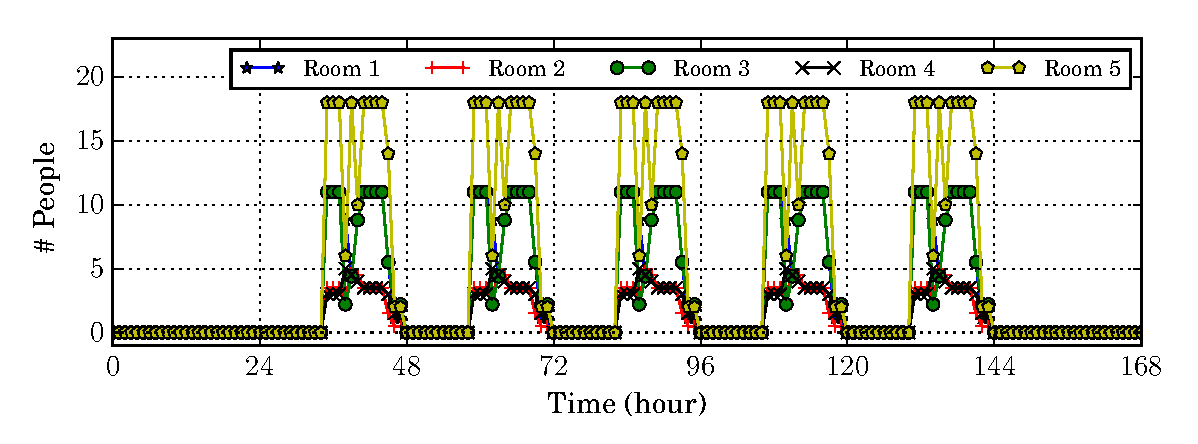
\includegraphics[width=0.9\columnwidth]{figs/energyplus_review/occupancy}
\caption{Occupancy information of 5 rooms during one week.}
\label{fig:occupancy-curve}
\end{figure}

We want to stress that fundamentally thermal behavior of building
systems is typically nonlinear (at least weakly nonlinear) due to the
temperature-dependent properties of the building materials and thermal
radiation effects. As a result, nonlinear modeling is preferred for accurate temperature
control and management.
